\documentclass{standalone}
\usepackage{tikz}
\usetikzlibrary{positioning}
\usetikzlibrary{decorations.pathmorphing}

\tikzset{snake it/.style={decorate, decoration={snake, segment length=1.5mm, amplitude=0.5mm}}}
\tikzset{
    position/.style args={#1:#2 from #3}{
        at=(#3.#1), anchor=#1+180, shift=(#1:#2)
    }
}

\begin{document}
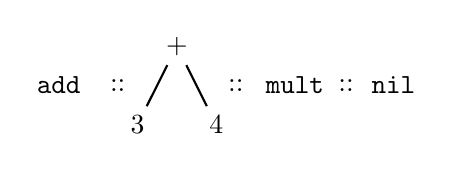
\begin{tikzpicture}
    \node (ADD) at (0.5,-1) {\texttt{add}};
    \node (CONS1) at (1.25,-1) {::};
    
    
    \node (PLUS) at (2,-0.5) {+};
    \node (THREE) at (1.5,-1.5) {3};
    \node (FOUR) at (2.5, -1.5) {4};
    \draw[thick] (PLUS) -- (THREE);
    \draw[thick] (PLUS) -- (FOUR);


    \node (CONS2) at (2.75,-1) {::};
    \node (MULT) at (3.5,-1) {\texttt{mult}};
    \node (CONS3) at (4.15,-1) {::};
    \node (NIL) at (4.75,-1) {\texttt{nil}};
    
    %\draw[help lines] (0,0) grid (20,-20);
\end{tikzpicture}
\end{document}